
\documentclass[12pt]{book}

\usepackage[norsk]{babel} 
\usepackage[utf8]{inputenc}
\usepackage{graphicx}

\usepackage{keystroke}
\usepackage{alltt}
\usepackage{fancyhdr}
\pagestyle{fancy}
\graphicspath{ {img/} }

\fancyhead{}
\fancyfoot{}


\begin{document}


\lhead{Andrew Roberts}
\rhead{\today}
\rfoot{\thepage}


\clearpage

\newcommand\nbvspace[1][3]{\vspace*{\stretch{#1}}}
\newcommand\nbstretchyspace{\spaceskip0.5em plus 0.25em minus 0.25em}
\newcommand{\nbtitlestretch}{\spaceskip0.6em}
\pagestyle{empty}
\begin{center}
\bfseries
\nbvspace[1]
\Huge
{\nbtitlestretch\huge
Gubberenn Dataprogram \\}

\nbvspace[10]
\normalsize

Bruksanvisning\\
GDPKonsoll\\

\nbvspace[2]

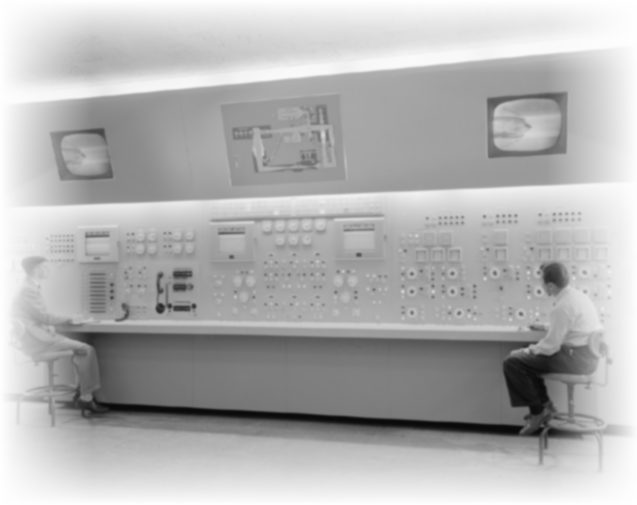
\includegraphics[width=5.0in]{gubb}
\nbvspace[15]
\normalsize

20(C)15\\
\large
Bjørkebakk og omegn Grendelag
\nbvspace[1]
\end{center}

\tableofcontents

\chapter{Bruksanvisning}

Hensikten med dette dokumentet er å forklare i detalj hvordan man kan bruke 'gubb-konsoll' -programmet på en Windows-plattform ala Windows 7 eller lignende. Programmet utfører de nødvendige beregningene i forbindelse med arrangeringen av Gubberennet. Beregningene er basert på ei input-fil som du oppretter ved hjelp av f.eks Microsoft Office Excel,  LibreOffice Calc eller et annet egnet regneark-program.  (Egentlig er det bare installeringen av 'gubb-konsoll' -programmet som er spesielt for Windows, bruken er den samme uavhengig av hvilken type datamaskin du har; Linux, Mac etc.)

\newpage

\section{Installasjon}

Aller først må du installere programmet. Dette gjør du ved å kjøre et program som heter GubbKonsollInstaller.exe Jeg forutsetter at du har fått tak i dette programmet, og at det ligger i en katalog som heter 'tmp' på en harddiskstasjon som heter 'C'. Siden GDPKonsoll er en konsollapplikasjon, skal du bare starte opp et kommandovindu først som sist. Dette gjør du ved å kjøre programmet 'cmd.exe'; klikk på Start-knappen, og skriv inn kommandoen i 'søk-feltet':

\begin{alltt}
\texttt{ cmd.exe  {\Return} }
\end{alltt}

Når du har fått opp kommandovinduet, går du til tmp-katalogen og kjører GunnKonsollInstaller.exe.

\begin{alltt}
\texttt{ cd c:/tmp/  {\Return} }

\texttt{ GubbKonsollInstaller.exe  {\Return} }
\end{alltt}

Dette skal resultere i at du får en rekke filer i en katalog som heter  'GubbKonsoll'  på "Skrivebordet". Gå dit:

\begin{alltt}
\texttt{ cd c:/Users/Ola Nordmann/Desktop/GubbKonsoll/  {\Return} }
\end{alltt}

Om du har en 'norsk' Windows-installasjon må du kanskje skrive noe slikt som dette:

\begin{alltt}
\texttt{ cd c:/Brukere/Ola Nordmann/Skrivebord/GubbKonsoll/  {\Return} }
\end{alltt}


Selve programmet heter gubb.exe Om du prøver å kjøre dette uten noen parametre, vil du få en oversikt over mulige kommandoer.

\begin{alltt}
\texttt{gubb.exe  {\Return} }

\texttt{BRUK: gubb [-i ARG] [-o ARG] [-l ARG] [-m ARG] [-r ARG] [-f ARG] [-hvbt]  }
\end{alltt}

De viktigste parametrene er '-i' og '-o'. Disse brukes til å angi ei inputfil, og ei outputfil. Inputfila må eksistere, mens outputfila opprettes av programmet.


\newpage

\section{Registrer data}

Blant de filene som ble installert, skal det ligge ei fil som heter 'testinput.csv'.  Kopier denne fila over til ei fil som du kaller for 'input.csv', slik:

\begin{alltt}
\texttt{copy testinput.csv input.csv  {\Return} }
\end{alltt}

Dette gjør vi primært for å ta vare på innholdet i testinput.csv -fila. Nå kan vi bruke 'input.csv' for å registrere årets data. Innholdet i 'input.csv' skal i utgangspunktet derfor se slik ut:

\scriptsize
\begin{alltt}
Startnummer;Herre-fornavn;Herre-etternavn;Dame-fornavn;Dame-etternavn;Start-tid;Slutt-tid;Oppgave-poeng
1;Eirik;Nordahl;Ester;Estensen;00:00:00;02:30:12;29,00
2;Jon;Johnsnen;Ann;Andersen;00:00:00;02:23:23;36,00
3;Kjell;Olson;Kari;Nordman;00:01:00;02:15:15;23,00
\end{alltt}

\normalsize

Denne fila åpner du i et egnet regne-ark-program. For de aller fleste vil dette være Microsoft Office Excel, men du kan godt bruke f.eks Libre Office Calc. Deretter blir all registrering av data kun en oppgave som dreier seg om å bruke et enkelt regneark. Formateringen av de ulike feltene er som følger:

\begin{itemize}
  \item Startnummer må være heltall
  \item Fornavn og etternavn er vanlig tekstfelt
  \item Start-tid og Slutt-tid angis som 'hh:mm:ss'
  \item Oppgave-poeng er desimaltall
\end{itemize}

Det første som registreres er de ulike navnene, etterhvert som folk kommer og melder seg på. Startnummer må velges vha loddtrekning eller lignende. Etterhvert som man begynner å fylle på med deltakere, kan man begynne å angi starttidspunkt for de ulike parene. Etterhvert som disse kommer i mål kan man angi mål-tidspunkt, og når oppgavene er rettet kan man registrere inn oppgave-poengene.

\newpage

\section{Utfør beregninger}

Da gjenstår det bare for gubb.exe å gjøre sin jobb, som er å beregne anvendt tid for hvert enkelt par, berenge idealtiden, beregne de ulike tidspoengene og til slutt sortere alle parene utfra oppnådd total-poeng-sum. Alt dette blir lagret til et nytt regneark som du oppgir navnet til, f.eks 'output.csv'

\begin{alltt}
\texttt{gubb.exe -i input.csv -o output.csv  {\Return} }
\end{alltt}

Nå kan du åpne output.csv i f.eks Excel og sjekk om beregningene er korrekte, og eventuelt gjøre videre databehandling i regnearket. Kanskje det mest aktuelle er bare å skrive det ut, slik at man har ei resultatliste til premieutdelinga.

\section{Skriv ut rapporter}

'gubb.exe' har funksjonalitet for å opprette noen rapporter som er identiske med de som Jan-Erik's dataprogram lager. Det dreier seg om ei startliste og to typer resultatlister, ei komplett og ei forenkla. Disse rapportene kan du lagre til tekst-filer, som igjen kan åpnes i notepad++.exe eller lignende for deretter å printe disse til en skriver. (notepad++ laster du gratis ned fra Internet) Du bør bruke Notepad++ siden denne editoren vil handtere øæå-problematikk korrekt, noe notepad.exe ikke gjør i utgangspunktet.


\begin{alltt}
\texttt{gubb.exe -i input.csv -o output.csv -r START -f start.txt  {\Return} }

\texttt{gubb.exe -i input.csv -o output.csv -r RES1 -f res1.txt  {\Return} }

\texttt{gubb.exe -i input.csv -o output.csv -r RES2 -f res2.txt  {\Return} }
\end{alltt}


\end{document}
